\documentclass[12pt]{article}
%\usepackage[utf8]{inputenc}
%\documentclass[UTF8]{ctexart}
%\usepackage[UTF8, heading = false, scheme = plain]{ctex}
\usepackage{geometry}
%geometry{a4paper,scale=0.9}
\geometry{a4paper,left=1cm,right=1cm,top=1cm,bottom=2cm}
\usepackage{amsfonts}
\usepackage{color}
\usepackage{url}
%\usepackage{biblatex}
\usepackage{amsmath}
\usepackage{amssymb}
\usepackage{latexsym}
\usepackage[linesnumbered,ruled,lined]{algorithm2e}
\usepackage{cite}
%\addbibresource{ref.bib}
%\bibliography{ref.bib}
\usepackage{caption}
\usepackage{graphicx, subfig}
\usepackage{float}
%\usepackage[fontset=ubuntu]{ctex}
%\usepackage{fontspec}
\usepackage{xeCJK}
%\usepackage[colorlinks,
%anchorcolor=black,
%citecolor=black]{hyperref}
%\setmainfont{SimSun}
\usepackage[section]{placeins}
\usepackage{enumitem}
\usepackage{framed}
\usepackage[framemethod=TikZ]{mdframed}
\usepackage{indentfirst}
\usepackage{setspace}%使用间距宏包
\linespread{1.5}

\title{在线最优化求解\cite{Online_Optimization}}
\author{leolinuxer}
%\date{June 2020}

\begin{document}
%\setlength{\parindent}{0pt}
\maketitle
\tableofcontents

\section{预备知识}
\subsection{凸函数}
略

\subsection{拉格朗日乘数法及 KKT 条件}
\subsubsection{常见的最优化问题分类}
(1) 无约束优化问题:
$$
X = \arg\min_Xf(X)
$$

含义是求解$X$,令目标函数$f(X)$最小;

(2) 有等式约束的优化问题:
$$
X = \arg\min_Xf(X)
$$
$$
s.t. \quad h_k(X) = 0; k = 1, 2, \cdots, n
$$

含义是在 $n$ 个等式约束$\{h_k(X)\}$ 的条件下,求解$X$,令目标函数$f(X)$最小;

(3)有不等式约束的优化问题:
$$
X = \arg\min_Xf(X)
$$
$$
s.t. \quad \begin{cases}
h_k(X) = 0; k = 1, 2, \cdots, n \\
g_l(X) \le 0; l = 1, 2, \cdots, m 
\end{cases}
$$

含义是在 $n$ 个等式约束$\{h_k(X)\}$以及 $m$ 个不等式约束$\{g_l(X)\}$的条件下,求解$X$,令 目标函数$f(X)$最小。

\subsubsection{针对无约束的最优化问题的解法}
针对无约束最优化问题,通常做法就是对$f(X)$求导,并令 $\frac{\partial }{\partial X}f(X) = 0$,求解可以得到最优值。如果$f(X)$为凸函数,则可以保证结果为全局最优解。

\subsubsection{针对有等式约束的最优化问题的解法}
针对有等式约束的最优化问题,采用\textbf{拉格朗日乘数法(Lagrange Multiplier)} 进行求解,通过拉格朗日系数$A = [a_1 , a_2, … , a_n ]^T \in \mathbb{R}^n $ 把等式约束和目标函数组合成为一个式子,对该式子进行最优化求解:
$$
X = \arg\min_X[f(X) + A^TH(X)]
$$

其中,$H(X) = [h_1(X), h_2(X), \cdots, h_n(X)]^T \in \mathbb{R}^n$,相当于将有等式约束的最优化问题转换成了 无约束最优化求解问题,解决方法依旧是对$f(X) + A^TH(X)$的各个参数$(X,A)$求偏导,并令其等于0,联立等式求解。

\subsubsection{针对有不等式约束的最优化问题的解法}
针对有不等式约束的最优化问题,常用的方法是\textbf{ KKT 条件(Karush-Kuhn-Tucker Conditions)},同样地,把所有的不等式约束、等式约束和目标函数全部写为一个式子:
$$
L(X,A,B) = f(X) + A^TH(X) + B^TG(X)
$$

KKT 条件是说最优值必须满足以下条件:
\begin{align*}
\frac{\partial}{\partial X} L(X,A,B) &= 0 \\
H(X) &= 0 \\
B^TG(X) &= 0\\
\end{align*}

其中,$B = [b_1, b_2, \cdots, b_m]^T \in \mathbb{R}^m$, $G(X) = [g_1(X), g_2(X), \cdots, g_m(X)]^T \in \mathbb{R}^m$;

KKT 条件是求解最优值$X^*$ 的必要条件,要使其成为充分必要条件,还需要$f(X)$为凸函数才行。

在 KKT 条件中,$B^TG(X) = 0$这个条件最有趣,因为$g_l(X) \le 0$,如果要满足这个等式,需要 $b_l = 0$或者 $g_l(X) = 0$。在我们后面的推导中会用到这个性质。

\subsection{从 Batch 到 Online}
我们面对的最优化问题都是无约束的最优化问题(有约束最优化问题可以利用拉格朗日乘数法或 KKT 条件转换成无约束最优化问题),因此我们通常可以将它们描述成:
\begin{align}
W &= \arg\min_W \ell(W,Z) \label{Eq_Optimize_W_Base}\\
Z &= \{(X_j, y_j) | j = 1, 2, \cdots, M\} \notag\\
y_j &= h(W, X_j) \notag
\end{align}

这里$Z$为观测样本集合(训练集);$X_j$为第 $j$ 条样本的特征向量;$y_j = h(W, X_j)$为预测值;$h(W, X_j)$为特征向量到预测值的映射函数;;$\ell(W,Z)$为最优化求解的目标函数,也称作损失函数,损失函数通常可以分解为各样本损失函数的累加,即$\ell(W,Z) = \sum_{j=1}^M\ell(W,Z_j)$;$W$为特征权重,也就是我们需要求解的参数。以线性回归和逻辑回归为例,它们的映射函数和损失函数分别为:
$$
\text{Linear Regression:}\qquad h(W,X_j) = W^TX_j  \qquad \ell(W,Z) = \sum_{j=1}^M(y_j - W^TX_j)^2
$$
$$
\text{Logistic Regression:}\qquad h(W,X_j) = \frac{1}{1 + e^{-W^TX_j}}  \qquad \ell(W,Z) = \sum_{j=1}^M\log(1 + e^{-y_jW^TX_j})
$$

在前面我们给出了无约束最优化问题解析解的求法。而在我们实际的数值计算中,通常做法是随机给定一个初始的$W(0)$ ,通过迭代,在每次迭代中计算损失函数在当前$W^{(t)}$的下降方向,并更新$W$,直到损失函数稳定在最小的点。例如著名的梯度下降法(GD, Gradient Descent)就是通过计算损失函数的在当前$W^{(t)}$ 处的梯度 (Gradient),以梯度$\triangledown_W\ell(W^{(t)},Z)$的 反方向作为下降方向更新$W$,如果损失函数是一个非平滑的凸函数(Non-smooth convex), 在不可导处用次梯度(Subgradient)方向的反方向作为下降方向。算法如下:
\begin{algorithm}  
\caption{Batch Gradient Descent}  
%\LinesNumbered
%\KwIn{}
%\KwOut{
Repeat until convergence \{ 

$\qquad \qquad W^{(t+1)} = W^{(t)} - \eta^{(t)} \triangledown_W\ell(W^{(t)}, Z)$

\}
\end{algorithm}  

GD 是一种批量处理的方式(Batch),每次更新$W$的时候都要扫描所有的样本以计算一个全局的梯度$\triangledown_W\ell(W,Z)$。

考虑另一种权重更新策略:
\begin{algorithm}  
\caption{Stochastic Gradient Descent}  
%\LinesNumbered
%\KwIn{}
%\KwOut{
Loop \{

\qquad for $j = 1$ to $M$ \{

$\qquad \qquad W^{(t+1)} = W^{(t)} - \eta^{(t)} \triangledown_W\ell(W^{(t)}, Z_j)$

\qquad \}

\}
\end{algorithm}  

在算法 2 中,每次迭代仅仅根据单个样本更新权重$W$,这种算法称作随机梯度下降(SGD, Stochastic Gradient Descent)。

与 GD 相比较,GD 每次扫描所有的样本以计算一个全局的梯度,SGD 则每次只针对一个观测到的样本进行更新。通常情况下,SGD 能够比 GD“更快”地令$W$逼近最优值。当样本数$M$特别大的时候,SGD 的优势更加明显,并且由于 SGD 针对观测到的“一条”样本更新 $W$,很适合进行增量计算,实现梯度下降的 Online 模式(OGD, Online Gradient Descent)。

\subsection{正则化}
正则化(Regularization)的意义本质上是为了避免训练得到的模型过度拟合(overfitting)训练数据。我们用图 2 来说明什么是过拟合,该图来自于王科的微博(@王小科科科)。图 2 是一个局部加权线性回归(Locally weighted linear regression)的训练结果,当学习度为 1 时,相当于进行线性回归,这时候模型与训练样本以及实际曲线拟合得都不够好,模型处于欠拟合(underfitting)状态;当学习度逐渐增加到 4 的过程中,模型逐渐与实际曲线吻合; 随着学习度继续增加,越来越多的样本直接落到模型曲线上(模型拟合训练数据),但是模型却与实际曲线相差越来越大,出现了过拟合。

\begin{figure}[H]
    \centering
    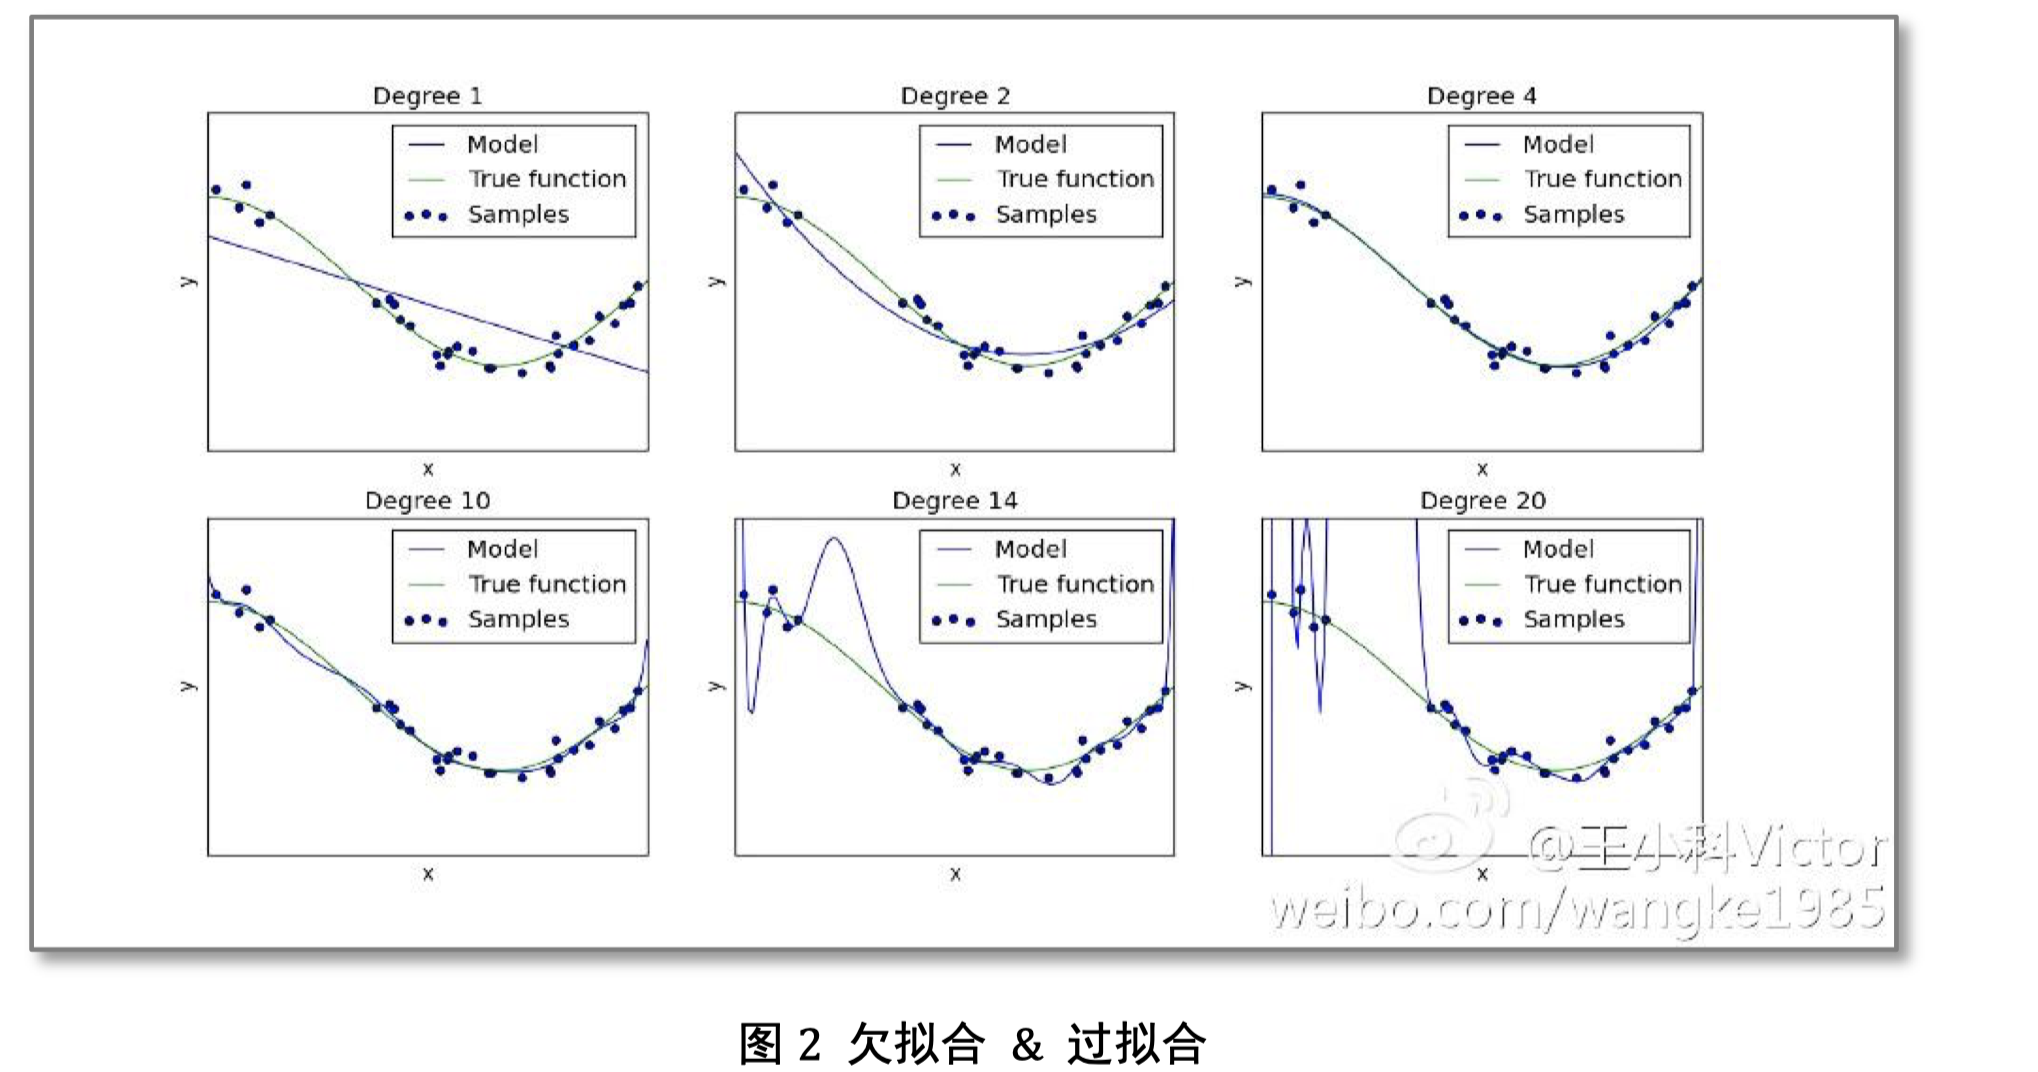
\includegraphics[width=.8\textwidth]{fig/OnlineOptimization-LearningDegree.png}
\end{figure}

\textcolor{red}{过拟合体现出来的现象就是特征权重$W$的各个维度的绝对值非常大}:一些大正数,一些大负数。这种模型虽然能够很好匹配样本(如图 2 中 Degree = 20 的情况),但是对新样本做预测的时候会使得预测值与真实值相差很远。

为了避免过拟合的情况,我们通常在损失函数的基础上加一个关于特征权重$W$的限制, 限制它的模不要太大,如果用$\psi(W)$表示特征权重$W$的一种求模计算,那么公式(\ref{Eq_Optimize_W_Base})转换成
\begin{align*}
W &= \arg\min_W \ell(W,Z) \\
& s.t. \quad \psi(W)  < \epsilon
\end{align*}

这个时候我们面对的是一个有约束的最优化问题。根据 KKT 条件,我们知道当选取合适的系数$\lambda$,那么这个有约束最优化问题等价于如下无约束最优化问题:
$$
W = \arg\min_W [\ell(W,Z) + \lambda\psi(W)]
$$

其中$\psi(W)$称作正则化因子(Regularizer),是一个关于$W$求模的函数,我们常用正则化因子有 L1 和 L2 正则化:
$$
\text{L1 Regularization}\qquad \psi(W) = ||W||_1 = \sum_{i=1}^N|w_i|
$$
$$
\text{L2 Regularization}\qquad \psi(W) = ||W||_2^2 = \sum_{i=1}^Nw_i^2 = W^TW
$$

不管是使用 L1 还是 L2 正则化,其基本原理都是一样的,即在最小化损失函数 $\ell(W,Z)$ 的同时,还要考虑$W$的模带来的贡献,从而避免$W$的维度上取一些绝对值很大的值。

L1 和 L2 正则化的区别主要有两个:(1) L1 正则化在 0 处不可导,而 L2 正则化可导。好在无论是 L1 还是 L2 正则化本身都是凸函数,因此在计算 L1 正则化的梯度方向的可以采用次梯度代替;(2) 在 Batch 模式下,L1 正则化通常产生更加稀疏(Sparse)的模型,$W$的更多维度为 0,这些为 0 的维度就代表了不是很相关的维度,从而起到了特征选择(Feature Selection)的目的。

L1正则化容易产生稀疏解的原因略。

那么在 Online 模式下呢,不同于 Batch,Online 中每次$W$的更新并不是沿着全局梯度进行下降,而是沿着某个样本的产生的梯度方向进行下降,整个寻优过程变得像是一个“随机” 查找的过程(SGD 中 Stochastic 的来历),这样 \textbf{Online 最优化求解即使采用 L1 正则化的方式, 也很难产生稀疏解}。

\begin{framed}
\textcolor{red}{理解 Online Optimization 算法和 SGD 算法的区别:}

在高维特征向量以及大数据集场景下,稀疏性很重要;

SGD 算法是随机查找最优梯度,即使采用 L1 正则化,也难以产生稀疏解;

因此,人们研究了在线最优化求解算法,用于更好地满足稀疏性。
\end{framed}

\section{在线最优化求解算法}
在前面我们做了一些热身,下面将针对在线最优化求解介绍一些算法。前文介绍了 L1 正则化在 Online 模式下也不能产生较好的稀疏性,而\textbf{稀疏性对于高维特征向量以及大数据集又特别的重要}。因此,我们沿着提升模型稀疏性的主线进行算法介绍。

\subsection{TG}
为了得到稀疏的特征权重$W$,最简单粗暴的方式就是设定一个阈值,当$W$的某维度上系数小于这个阈值时将其设置为 0(称作简单截断)。这种方法实现起来很简单,也容易理解。 但实际中(尤其在 OGD 里面)$W$的某个系数比较小可能是因为该维度训练不足引起的,简单进行截断会造成这部分特征的丢失。

截断梯度法(TG, Truncated Gradient)是由 John Langford,Lihong Li 和 Tong Zhang 在 2009 年提出 [10] ,实际上是对简单截断的一种改进。下面首先描述一下 L1 正则化和简单截断的方法,然后我们再来看 TG 对简单截断的改进以及这三种方法在特定条件下的转化。

\subsubsection{L1 正则化法}
由于 L1 正则项在 0 处不可导,往往会造成平滑的凸优化问题变成非平滑凸优化问题, 因此在每次迭代中采用次梯度计算 L1 正则项的梯度。权重更新方式为:
$$
W^{(t+1)} = W^{(t)} - \eta^{(t)}G^{(t)} - \eta^{(t)}\lambda sgn(W^{(t)})
$$

注意, 这里$\lambda \in \mathbb{R}$是一个标量, 且$\lambda \ge 0$, 为 L1 正则化参数;$sgn(v)$)为符号函数,如果$V = [v_1, v_2, \cdots, v_N] \in \mathbb{R}^N$是 一 个 向 量,$v_i$是 向 量 的一个维度,那么有$sgn(V) = [sgn(v_1), sgn(v_2), \cdots, sgn(v_N)] \in \mathbb{R}^N$;$\eta^{(t)}$为学习率,通常将其设置成$1/\sqrt{t}$的函数;$G^{(t)} = \triangledown_W\ell(W^{(t)}, Z^{(t)})$代表了第$t$次迭代中损失函数的梯度,由于 OGD 每次仅根据观测到的一个样本进行权重更新,因此也不再使用区分样本的下标$j$。

\subsubsection{简单截断法}
以$k$为窗口,当$t/k$不为整数时采用标准的 SGD 进行迭代;当$t/k$为整数时,采用如下权重更新方式(也就是说,每间隔$k$步,进行一次截断操作):
$$
W^{(t+1)} = T_0(W^{(t)} - \eta^{(t)}G^{(t)}, \theta)
$$
\begin{equation}
T_0(v_i, \theta) = \begin{cases}
0 \qquad if \ |v_i| \le \theta \\
v_i \qquad otherwise
\end{cases} \label{Eq_Simple_Truancate}
\end{equation}


注意,这里面$\theta \in \mathbb{R}$是一个标量,且$\theta \ge 0$;如果$V = [v_1, v_2, \cdots, v_N] \in \mathbb{R}^N$是一个向量,$v_i$是向量的一个维度,那么有$T_0(V, \theta) = [T_0(v_1,\theta), T_0(v_2, \theta), \cdots, T_0(v_N, \theta)] \in \mathbb{R}^N$。

\subsubsection{截断梯度法(TG)}
上述的简单截断法被 TG 的作者形容为 too aggressive,因此 TG 在此基础上进行了改进,同样是采用截断的方式,但是比较不那么粗暴。采用相同的方式表示为:
$$
W^{(t+1)} = T_1(W^{(t)} - \eta^{(t)}G^{(t)}, \eta^{(t)}\lambda^{(t)}, \theta)
$$
\begin{equation}
T_1(v_i, \alpha, \theta) = \begin{cases}
\max(0, v_i - \alpha) \qquad if \ v_i \in [0, \theta] \\
\min(0, v_i + \alpha) \qquad if \ v_i \in [-\theta, 0] \\
v_i \qquad otherwise
\end{cases} \label{Eq_TG}
\end{equation}

其中$\lambda^{(t)} \in \mathbb{R}$ 且$\lambda^{(t)} \ge 0$。TG 同样是以$k$为窗口,每$k$步进行一次截断。当$t/k$不为整数时$\lambda^{(t)} = 0$,当$t/k$为整数时$\lambda^{(t)} = k\lambda$。从公式(\ref{Eq_TG})可以看出,$\lambda$和$\theta$决定了$W$的稀疏程度,这两个值越大,则稀疏性越强。尤其令$\lambda = \theta$时,只需要通过调节一个参数就能控制稀疏性。

根据公式(\ref{Eq_TG}),我们很容易写出 TG 的算法逻辑:
\begin{algorithm}  
\caption{Batch Gradient Descent}  
%\LinesNumbered
\KwIn{$\theta$}
\KwOut{$W$}

\textbf{Initial $W \in \mathbb{R}^N$}

\For{ $t = 1, 2, 3, \cdots$ }{
	$G = \triangledown_W\ell(W, X^{(t)}, y^{(t)})$ \newline
	refresh $W$ according to \newline
	$w_i = \begin{cases}
		\max(0, w_i - \eta^{(t)}g_i - \eta^{(t)}\lambda^{(t)}) \qquad if \ (w_i - \eta^{(t)}g_i) \in [0, \theta] \\
		\min(0, w_i - \eta^{(t)}g_i + \eta^{(t)}\lambda^{(t)}) \qquad if \ (w_i - \eta^{(t)}g_i) \in [-\theta, 0] \\
		w_i - \eta^{(t)}g_i \qquad otherwise 
	\end{cases}$
}
\end{algorithm}  

\subsubsection{TG 与简单截断以及 L1 正则化的关系}
简单截断和截断梯度的区别在于采用了不同的截断公式$T_0$ 和$T_1$ ,如图所示。
\begin{figure}[H]
    \centering
    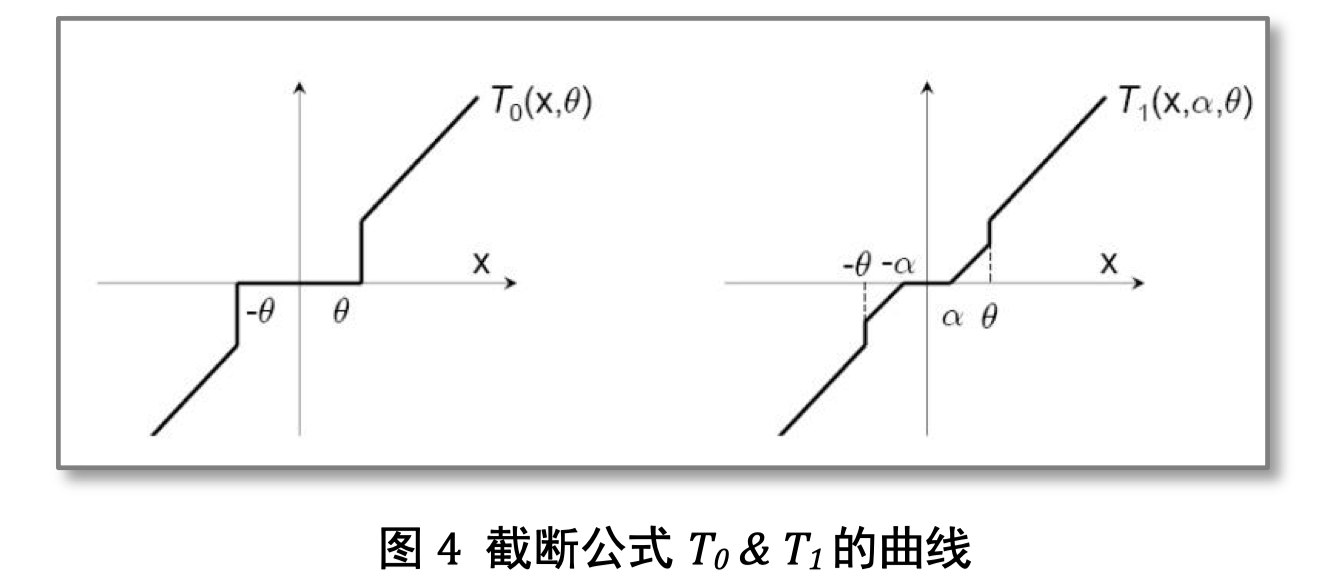
\includegraphics[width=.8\textwidth]{fig/OnlineOptimization-T0T1.png}
\end{figure}

为了清晰地进行比较,我们将公式(\ref{Eq_TG})进行改写,描述特征权重每个维度的更新方式:
$$
w_i^{(t+1)} = \begin{cases}
Trnc\big((w_i^{(t)} - \eta^{(t)}g_i^{(t)}), \lambda_{TG}^{(t)}, \theta\big) \qquad if \ mod(t, k) = 0 \\
w_i^{(t)} - \eta^{(t)}g_i^{(t)} \qquad \qquad \qquad \qquad \quad otherwise
\end{cases}
$$
$$
\lambda_{TG}^{(t)} = \eta^{(t)}\lambda k
$$
$$
Trnc\big( w, \lambda_{TG}^{(t)}, \theta \big) = \begin{cases}
0 \qquad \qquad \qquad \qquad if \ |w| \le \lambda_{TG}^{(t)} \\
w - \lambda_{TG}^{(t)} sgn(w) \qquad if \ \lambda_{TG}^{(t)} \le |w| \le \theta \\
w \qquad \qquad \qquad \qquad otherwise
\end{cases}
$$

如果令$\lambda_{TG}^{(t)} = \theta$,截断公式$Trnc\big( w, \lambda_{TG}^{(t)}, \theta \big)$变成:
$$
Trnc\big(w, \theta, \theta \big) = \begin{cases}
0 \quad if \ |w| \le \theta \\
w \quad otherwise
\end{cases}
$$
此时 TG 退化成简单截断法。

如果令$\theta = \infty$,截断公式$Trnc\big( w, \lambda_{TG}^{(t)}, \theta \big)$变成:
$$
Trnc\big(w, \lambda_{TG}^{(t)}, \infty \big) = \begin{cases}
0 \qquad \qquad \qquad \quad if \ |w| \le \lambda_{TG}^{(t)} \\
w - \lambda_{TG}^{(t)} sgn(w)  \quad otherwise
\end{cases}
$$
如果再令$k= 1$,即每步都截断,那么特征权重维度更新公式变成
$$
w_i^{(t+1)} = \begin{cases}
Trnc\big((w_i^{(t)} - \eta^{(t)}g_i^{(t)}), \eta^{(t)}\lambda, \infty \big)  = w_i^{(t)} - \eta^{(t)}g_i^{(t)} - \eta^{(t)}\lambda sgn(w_i^{(t)}) \qquad if \ |w| \ge \lambda_{TG}^{(t)} \\
0 \qquad otherwise
\end{cases}
$$
此时 TG 退化成 L1 正则化法。

\subsection{FOBOS}
\subsubsection{FOBOS 算法原理}
前向后向切分(FOBOS, Forward-Backward Splitting)是由 John Duchi 和 Yoram Singer 提出的 [11] 。从全称上来看,该方法应该叫 FOBAS,但是由于一开始作者管这种方法叫 FOLOS (Forward Looking Subgradients),为了减少读者的困扰,作者干脆只修改一个字母,叫 FOBOS。

在 FOBOS 中,将权重的更新分为两个步骤:


%\printbibliography
\bibliography{../ref}
\bibliographystyle{IEEEtran}
\end{document}